% ==============================================================================
% 4. DESENVOLVIMENTO
% ==============================================================================
\chapter{Desenvolvimento}
\label{cap:desenvolvimento}

\section{Código-alvo}
\label{sec:alvo}

O código-alvo é um avaliador de expressões em TypeScript, escrito para suportar cláusulas no estilo do \texttt{WHERE} do SQL: comparações (\texttt{=}, \texttt{<>}, \texttt{<}, \texttt{<=}, \texttt{>}, \texttt{>=}), aritmética (\texttt{+}, \texttt{-}, \texttt{*}, \texttt{/}), operadores lógicos (\texttt{and}, \texttt{or}), \texttt{is [not] null}, \texttt{between}, expressões \texttt{case when \ldots then \ldots else \ldots end}, chamadas de função (\texttt{length}), literais numéricos, de texto e booleanos, identificadores resolvidos por um contexto e agrupamento por parênteses. Ele tem 622 linhas em cinco arquivos: \texttt{lexer.ts} (206 linhas), que converte o texto em \textit{tokens}; \texttt{parser.ts} (221), um \textit{parser} de precedência de operadores que produz uma árvore sintática; \texttt{evaluator.ts} (89), que percorre a árvore e calcula o valor; e \texttt{ast.ts} (52) e \texttt{token.ts} (54), que só definem tipos. A API pública tem três funções: \texttt{parse(expression)}, \texttt{evaluate(expression, context?)} e \texttt{evaluateObject(expression, value)}.

A escolha é deliberada. O alvo é lógica pura e determinística, sem E/S, sem dependências e sem estado compartilhado, o que elimina fontes de variação alheias à suíte. É pequeno o bastante para que um teto possa ser construído e \textbf{demonstrado} (cada mutante sobrevivente pode ser analisado um a um), e rico o bastante para ser difícil de testar bem: há precedência de operadores, fronteiras de classes de caracteres no \textit{lexer}, tratamento de fim de entrada, mensagens de erro com posição e vários caminhos de erro sintático. O StrykerJS gera 369 mutantes válidos nos três arquivos de lógica (177 no \textit{lexer}, 92 no \textit{parser}, 100 no avaliador), dominados por expressões condicionais (138), remoção de blocos (77), literais de texto (50) e operadores de igualdade (47).

\section{Aparato de avaliação}
\label{sec:aparato}

O aparato separa o que a LLM vê do que a julga. O repositório \texttt{bench} contém apenas o código-alvo, um \texttt{package.json} com o Vitest e uma configuração mínima de teste; é um projeto comum que precisa de testes. O repositório \texttt{validator} contém tudo o mais: os prompts, a suíte do teto, cada suíte gerada, o \textit{script} de pontuação, a configuração do Stryker e os detectores do SNUTS.js. Um \textit{script} verifica, por \textit{hash}, que o código mutado é byte a byte o mesmo que a LLM testou. Antes de cada geração, o \texttt{bench} é copiado para um diretório com nome neutro e sem histórico, para que nem o caminho nem o \texttt{git log} revelem que existe um avaliador.

A pontuação de uma suíte segue sempre o mesmo caminho: (1) o Vitest executa a suíte sobre o código correto, com cobertura por V8 restrita aos três arquivos de lógica e com emissão de cobertura mesmo quando há falhas, e registra quais casos de teste falharam; (2) os casos que falharam são marcados como ignorados numa cópia da suíte, usada apenas na etapa seguinte; (3) o StrykerJS roda a cópia contra os 369 mutantes, com análise de cobertura por teste; (4) os detectores do SNUTS.js contam \textit{smells} na suíte original; (5) as métricas da seção ``\nameref{sec:metricas}'' e as distâncias até o teto são calculadas e gravadas em JSON. Nada é corrigido à mão em nenhuma etapa.

\subsection{Um achado sobre a execução em paralelo}
\label{sec:timeout}

A primeira versão do \textit{script} pontuava várias suítes ao mesmo tempo, cada uma com seu próprio processo do Stryker, que por sua vez abre vários processos de trabalho. Numa rodada-piloto com seis suítes de modelos anteriores, executada assim, o teto de então marcou 95,1\% de escore de mutação. Pontuado de novo, sozinho, no mesmo ambiente, ele marcou 92,7\%. A diferença estava inteiramente nos \textit{timeouts}: 95 mutantes na execução paralela contra 29 na sequencial. O Stryker calcula o tempo-limite de cada mutante a partir de uma execução de referência; quando a máquina está sob carga, mutantes que apenas tornam o código mais lento, sem impedir que termine, estouram o limite e são contados como mortos. Nas seis suítes de LLM do piloto, repontuadas em sequência, a inflação variou de 0,5 a 5,4 pontos percentuais e não foi uniforme: a distância de uma mesma suíte até o teto, que era de 5,1 pontos na pontuação paralela, passou a 13,3 pontos na sequencial, porque teto e suíte tinham sido inflados em medidas diferentes.

A consequência prática é que escores de mutação obtidos em execuções paralelas não são comparáveis entre si nem com execuções isoladas, e são sistematicamente otimistas. Toda a pontuação deste estudo é sequencial, e as tabelas reportam mutantes mortos e por \textit{timeout} em colunas separadas. Os 29 \textit{timeouts} que restam na execução sequencial correspondem a mutações que de fato removem a condição de parada de laços do \textit{lexer} e do \textit{parser}, e são detecções legítimas.

\section{Construção e revisão do teto}
\label{sec:teto}

O teto foi construído em duas fases. Na primeira, uma suíte foi escrita com apoio de LLM e refinada a partir dos relatórios do Stryker e do SNUTS.js até o escore saturar, chegando a 104 testes, cobertura de 99,2\% de linhas e 97,3\% de ramos, nenhum \textit{smell} e, medida sequencialmente, 92,7\% de escore de mutação, com 21 mutantes sobreviventes e 6 sem cobertura.

Na segunda fase, cada um desses 27 mutantes foi analisado individualmente. O resultado mudou a leitura do que a primeira fase tinha produzido: dos 21 sobreviventes, 19 eram matáveis. Eram, quase todos, casos de fronteira que a suíte original não exercitava: o dígito \texttt{9}, limite superior da faixa numérica do \textit{lexer} (a suíte usava 0 a 8 e não percebia que a mutação \texttt{<= 0x39} $\to$ \texttt{< 0x39} tornava \texttt{9} um caractere ilegal); um número decimal com mais de um dígito antes do ponto (\texttt{12.5}), porque com um dígito só a mutação na guarda do ponto decimal é indistinguível; identificadores começando por \texttt{A}, \texttt{Z} e \texttt{z}, os limites das faixas de letras; os caracteres \texttt{[} e \texttt{\{}, imediatamente após \texttt{Z} e \texttt{z}, que devem ser ilegais; o cálculo da posição do \textit{token}, que só é observável nas mensagens de erro e que a suíte verificava com expressões regulares parciais; e a guarda de \texttt{case} sem \texttt{when}, que só é distinguível com a entrada \texttt{case end}. Doze testes, um comportamento por teste, mataram os 19. A suíte final tem 116 testes, 97,8\% de escore de mutação (332 mutantes mortos, 29 por \textit{timeout}, 2 sobreviventes, 6 sem cobertura), mesma cobertura e nenhum \textit{smell}.

Os oito mutantes restantes têm, cada um, um argumento de por que nenhum teste pode matá-los, registrado no Apêndice~\ref{ap:equivalentes}. Dois são equivalentes no sentido clássico: o valor inicial de um campo que o construtor reatribui antes de qualquer leitura, e o valor de fim de entrada devolvido por \texttt{peekChar}, que só é usado em comparações nas quais \texttt{""} e \texttt{'\textbackslash 0'} se comportam igual. Seis são código inalcançável pela API pública: um \texttt{if} cuja condição nunca é verdadeira porque a função chamada retorna um objeto ou lança exceção, e dois ramos \texttt{default} de \textit{switches} para operadores e tipos de nó que o \textit{parser} nunca produz. As linhas não cobertas pela suíte (99,2\% de linhas) são exatamente essas, então a cobertura do teto também é a máxima alcançável pela API pública. Subtraindo os oito do denominador, o teto atinge 100\%; mantendo-os, como fazemos para todas as suítes, 97,8\% é o limite superior para este alvo.

Duas lições ficam dessa fase. A primeira é que uma suíte construída com LLM, ferramentas e iteração, e que parecia saturada, ainda deixava 19 mutantes matáveis em fronteiras de classes de equivalência; o que a tornou um teto não foi o processo de construção, foi a análise individual dos sobreviventes. A segunda é que ``teto'' é uma afirmação sobre o alvo, não sobre quem o construiu, e por isso ela precisa vir acompanhada de prova: sem a classificação dos sobreviventes, qualquer distância medida contra a referência carrega uma incerteza que não se consegue quantificar.

\section{Condições experimentais e geração}
\label{sec:condicoes}

A \autoref{tab:modelos} lista os modelos. Os três foram usados na mesma condição de interface: uma única mensagem contendo o prompt da condição e o projeto-alvo, sem execução de testes, sem segunda rodada e sem correção. Para o modelo acessado por ferramenta de codificação, isso foi obtido executando a ferramenta em modo não interativo com as ferramentas de leitura e escrita de arquivos habilitadas e a execução de comandos desabilitada: o modelo lê os arquivos do projeto e escreve o arquivo de testes, e só. Para o modelo acessado por aplicativo de chat e para o acessado por API, o conteúdo dos cinco arquivos do projeto e da configuração do Vitest foi incluído na própria mensagem, logo após o prompt, com os mesmos caminhos relativos. O texto dos prompts é idêntico nas três interfaces e consta no Apêndice~\ref{ap:prompts}; P2 acrescenta a P1 uma seção ``critérios de qualidade'' que nomeia cobertura, poder de detecção (com instrução de afirmar valores exatos e testar fronteiras) e manutenibilidade (com os \textit{smells} a evitar).

\begin{table}[htb]
    \centering
    \ABNTEXfontereduzida
    \begin{minipage}{\textwidth}
        \caption{Modelos avaliados e forma de acesso}
        \label{tab:modelos}
        \centering
        \begin{tabular}{p{1.6cm}p{5.2cm}p{3.6cm}p{4.4cm}}
            \toprule
            \textbf{Rótulo} & \textbf{Modelo} & \textbf{Acesso} & \textbf{Configuração} \\
            \midrule
            Fable & Claude Fable 5.1 (Anthropic) & Claude Code, modo não interativo & leitura/escrita de arquivos; sem execução de comandos \\
            Gemini & \pendente{nome exato exibido no app} (Google) & aplicativo de chat & sessão nova por geração; memória desligada \\
            DeepSeek & DeepSeek V4.1 Flash (\texttt{deepseek-v4.1-flash-1017}) & API (OpenRouter) & parâmetros padrão da API \\
            \bottomrule
        \end{tabular}
        \legend{Fonte: Própria do autor (2026).}
    \end{minipage}
\end{table}

Cada condição foi gerada cinco vezes, cada vez numa sessão nova e numa cópia nova do projeto. As gerações por API e por ferramenta de codificação foram automatizadas por \textit{scripts} que também registram data, duração e, quando a API informa, o número de \textit{tokens} de saída; as gerações pelo aplicativo de chat foram feitas manualmente, com a mesma mensagem, e a resposta completa foi guardada ao lado do arquivo de testes extraído. Suítes que não executam (por erro de importação ou de sintaxe) são mantidas e reportadas como tal. \pendente{Registrar aqui quantas, se houver.}

\section{Resultados}
\label{sec:resultados}

\pendente{Seção a preencher com os dados do experimento. As tabelas e figuras abaixo são geradas automaticamente a partir de \texttt{results/results.json} pelo script de análise; o texto será escrito sobre os números finais.}

\subsection{Distância até o teto (QP1 e QP3)}

\IfFileExists{tabelas/tab_consolidada.tex}{\begin{table}[htb]
    \centering
    \ABNTEXfontereduzida
    \begin{minipage}{\textwidth}
        \caption{Teto e condições: média $\pm$ desvio padrão das gerações pontuadas}
        \label{tab:consolidada}
        \centering\scriptsize\setlength{\tabcolsep}{3pt}
        \begin{tabular}{llr rr rr rrr r}
            \toprule
            \textbf{Condição} & \textbf{Prompt} & $n$ & \textbf{Testes} & \textbf{FP} & \textbf{Cob.L} & \textbf{Cob.R} & $R$ & $P$ & $F_1$ & \textbf{Smells/teste} \\
            \midrule
            Teto & -- & 1 & 119 & 0 & 100,0 & 99,3 & 99,5 & 100,0 & 99,7 & 0,00 \\
            \midrule
            Fable & P1 & 5 & 118 & 0,0 & 98,4 $\pm$ 0,3 & 96,0 $\pm$ 0,5 & 91,1 $\pm$ 0,4 & 100,0 $\pm$ 0,0 & 95,3 $\pm$ 0,2 & 0,09 $\pm$ 0,06 \\
            Fable & P2 & 5 & 164 & 0,8 & 99,2 $\pm$ 0,3 & 97,5 $\pm$ 0,7 & 95,9 $\pm$ 0,5 & 99,5 $\pm$ 0,6 & 97,7 $\pm$ 0,1 & 0,03 $\pm$ 0,02 \\
            DeepSeek & P1 & 5 & 28 & 0,2 & 97,0 $\pm$ 1,1 & 92,2 $\pm$ 3,1 & 81,6 $\pm$ 2,5 & 99,6 $\pm$ 0,9 & 89,7 $\pm$ 1,6 & 0,04 $\pm$ 0,08 \\
            DeepSeek & P2 & 5 & 90 & 0,2 & 99,3 $\pm$ 0,2 & 97,6 $\pm$ 0,6 & 94,6 $\pm$ 1,6 & 99,8 $\pm$ 0,5 & 97,1 $\pm$ 0,9 & 0,02 $\pm$ 0,02 \\
            \bottomrule
        \end{tabular}
        \legend{Fonte: Própria do autor (2026). Cobertura, $R$, $P$ e $F_1$ em \%; $n$ = gerações pontuadas.}
    \end{minipage}
\end{table}
}{\pendente{Tabela consolidada: teto e, para cada condição, média $\pm$ desvio das cinco gerações em testes, FP, Cob.L, Cob.R, R, P, F$_1$ e smells/teste.}}

\IfFileExists{tabelas/tab_gaps.tex}{\begin{table}[htb]
    \centering
    \ABNTEXfontereduzida
    \begin{minipage}{\textwidth}
        \caption{Distância média até o teto por dimensão (teto $-$ condição), com IC 95\% por \textit{bootstrap}}
        \label{tab:gaps}
        \centering\scriptsize\setlength{\tabcolsep}{3pt}
        \begin{tabular}{ll rrrrrr}
            \toprule
            \textbf{Condição} & \textbf{Prompt} & $\Delta$Cob.L & $\Delta$Cob.R & $\Delta R$ & $\Delta P$ & $\Delta F_1$ & $\Delta$Smells \\
            \midrule
            Fable & P1 & 1,6 [1,3; 1,8] & 3,3 [2,9; 3,8] & 8,4 [8,1; 8,7] & 0,0 [0,0; 0,0] & 4,4 [4,2; 4,6] & 0,09 [0,04; 0,13] \\
            Fable & P2 & 0,8 [0,5; 1,0] & 1,8 [1,2; 2,4] & 3,6 [3,1; 3,9] & 0,5 [0,1; 0,9] & 2,1 [2,0; 2,2] & 0,03 [0,02; 0,05] \\
            Gemini & P1 & 1,7 [1,6; 1,9] & 3,6 [3,3; 3,9] & 8,7 [7,8; 9,8] & 2,0 [0,5; 3,6] & 5,5 [4,2; 6,8] & 0,01 [0,00; 0,03] \\
            Gemini & P2 & 0,9 [0,8; 1,0] & 2,1 [2,0; 2,4] & 2,2 [1,9; 2,6] & 0,3 [0,0; 0,7] & 1,3 [1,0; 1,7] & 0,01 [0,01; 0,01] \\
            DeepSeek & P1 & 3,0 [2,1; 4,0] & 7,2 [5,0; 9,8] & 17,9 [15,9; 19,9] & 0,4 [0,0; 1,2] & 10,1 [8,8; 11,3] & 0,04 [0,00; 0,12] \\
            DeepSeek & P2 & 0,7 [0,5; 0,8] & 1,8 [1,2; 2,0] & 4,9 [3,6; 6,1] & 0,2 [0,0; 0,7] & 2,6 [1,9; 3,3] & 0,02 [0,01; 0,04] \\
            \bottomrule
        \end{tabular}
        \legend{Fonte: Própria do autor (2026). Valores positivos = abaixo do teto; para smells o sinal é invertido (positivo = mais smells que o teto).}
    \end{minipage}
\end{table}
}{\pendente{Tabela de distâncias: $\Delta$ médio por condição e por dimensão, com IC 95\%.}}

\IfFileExists{figuras/fig_r_por_condicao.pdf}{%
\begin{figure}[htb]
    \centering
    \begin{minipage}{0.9\textwidth}
        \caption{\label{fig:r-condicao}Escore de mutação das cinco gerações de cada condição, com o teto como referência}
        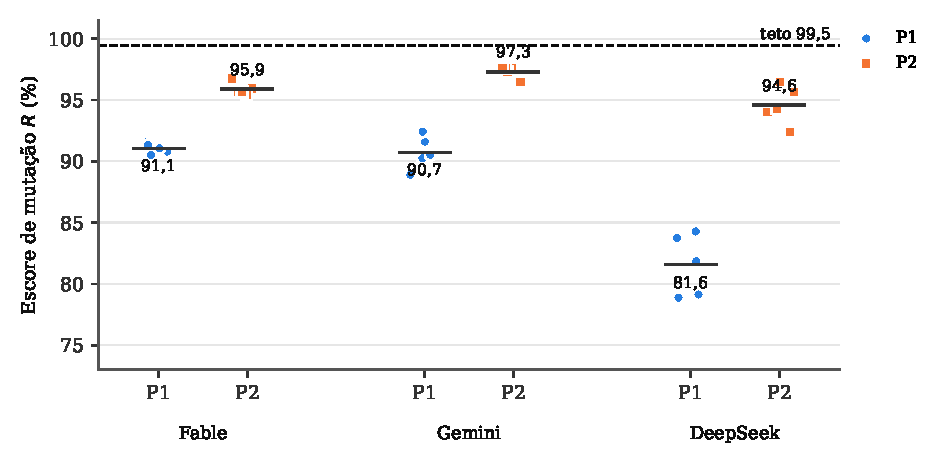
\includegraphics[width=\textwidth]{figuras/fig_r_por_condicao.pdf}
        \par
        \legend{Fonte: Própria do autor (2026).}
    \end{minipage}
\end{figure}}{\pendente{Figura: escore de mutação das cinco gerações por condição, com a linha do teto.}}

\pendente{Texto da QP1: distância média por modelo e por dimensão; destacar a diferença entre cobertura e escore de mutação. Texto da QP3: em qual dimensão a distância é maior, e se isso vale para os três modelos.}

\subsection{Efeito do prompt ciente das métricas (QP2)}

\IfFileExists{figuras/fig_gap_dimensao.pdf}{%
\begin{figure}[htb]
    \centering
    \begin{minipage}{0.9\textwidth}
        \caption{\label{fig:gap-dimensao}Distância média até o teto por dimensão, P1 e P2, por modelo}
        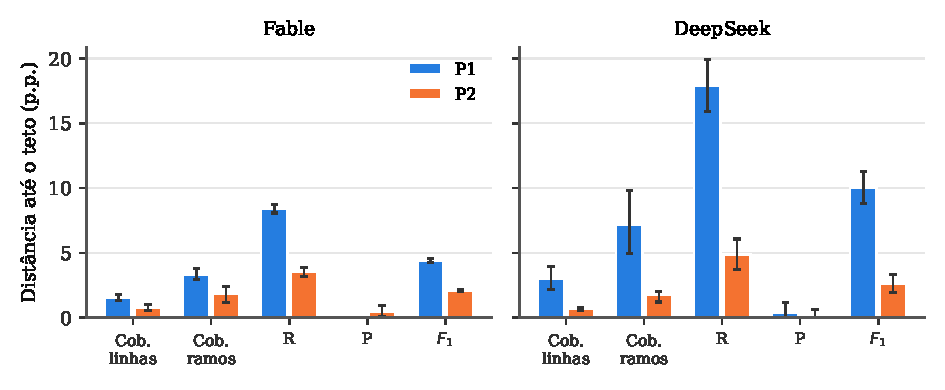
\includegraphics[width=\textwidth]{figuras/fig_gap_dimensao.pdf}
        \par
        \legend{Fonte: Própria do autor (2026).}
    \end{minipage}
\end{figure}}{\pendente{Figura: distância por dimensão, P1 vs P2, por modelo.}}

\pendente{Texto da QP2: redução média da distância com P2 por modelo e por métrica; delta de Cliff; o que mudou nas suítes (mais testes? asserções exatas? menos smells?).}

\subsection{Estabilidade entre gerações (QP4)}

\IfFileExists{tabelas/tab_estabilidade.tex}{\begin{table}[htb]
    \centering
    \ABNTEXfontereduzida
    \begin{minipage}{\textwidth}
        \caption{Estabilidade entre gerações: dispersão do escore de mutação por condição}
        \label{tab:estabilidade}
        \centering\scriptsize\setlength{\tabcolsep}{3pt}
        \begin{tabular}{ll rrr r r r r}
            \toprule
            \textbf{Condição} & \textbf{Prompt} & $\bar{R}$ & dp & CV (\%) & mín.--máx. & IC 95\% & $k^*$ & dp $F_1$ \\
            \midrule
            Fable & P1 & 91,1 & 0,4 & 0,5 & 90,5--91,6 & $\pm$0,4 & 1 & 0,2 \\
            Fable & P2 & 95,9 & 0,5 & 0,5 & 95,4--96,7 & $\pm$0,5 & 1 & 0,1 \\
            Gemini & P1 & 90,7 & 1,3 & 1,5 & 88,9--92,4 & $\pm$1,2 & 2 & 1,7 \\
            Gemini & P2 & 97,3 & 0,5 & 0,5 & 96,5--97,6 & $\pm$0,4 & 1 & 0,5 \\
            DeepSeek & P1 & 81,6 & 2,5 & 3,1 & 78,9--84,3 & $\pm$2,2 & 7 & 1,6 \\
            DeepSeek & P2 & 94,6 & 1,6 & 1,7 & 92,4--96,5 & $\pm$1,4 & 3 & 0,9 \\
            \bottomrule
        \end{tabular}
        \legend{Fonte: Própria do autor (2026). Concordância do ordenamento completo das condições por $R$ ao tomar uma geração ao acaso por condição: 49,7\% das amostras reproduzem o ordenamento pelas médias ($\tau$ médio de Kendall = 0,89). $k^*$: gerações necessárias para semi-amplitude de 2,0 p.p. no IC 95\% de $R$.}
    \end{minipage}
\end{table}
}{\pendente{Tabela de estabilidade: por condição, desvio padrão e coeficiente de variação de R e de F$_1$, amplitude (mín.--máx.), semi-amplitude do IC 95\% e $k$ necessário para semi-amplitude de 2 p.p.}}

\pendente{Texto da QP4: quanto varia; se o ordenamento das condições se mantém ao tomar uma geração ao acaso (fração de concordância); quantas gerações seriam necessárias; conclusão sobre avaliações de geração única.}

\section{Discussão}
\label{sec:discussao}

\pendente{Discussão a escrever sobre os resultados finais. Pontos já definidos pela estrutura do estudo:}

\begin{itemize}
    \item \pendente{Cobertura alta com escore de mutação menor: o que isso diz sobre as asserções geradas (relação com o problema do oráculo de \citeonline{konstantinou2024}).}
    \item \pendente{O que P2 compra e o que não compra: se o prompt fecha parte da distância, é evidência de que o modelo sabe fazer melhor quando sabe o que será medido; se não fecha, é evidência de limite de capacidade e não de informação.}
    \item \pendente{Custo: o modelo de baixo custo em relação aos de fronteira, por ponto percentual de distância.}
    \item \pendente{Se alguma geração alcançar ou superar o teto em alguma métrica: o teto é uma afirmação sobre o alvo e precisa ser revisado quando os recursos melhoram; discutir o que a suíte fez para chegar lá.}
    \item Metodológico: o achado dos \textit{timeouts} (seção ``\nameref{sec:timeout}'') vale para qualquer estudo que use Stryker ou ferramentas com limite de tempo adaptativo em execução paralela, e a revisão do teto (seção ``\nameref{sec:teto}'') mostra que ``saturou'' não é o mesmo que ``máximo''.
    \item \pendente{Implicações para a prática: usar teste de mutação como portão para testes gerados; incluir os critérios no prompt; gerar mais de uma vez e selecionar (custo de \textit{best-of-k} em relação ao ganho observado).}
\end{itemize}

\section{Ameaças à validade}
\label{sec:ameacas}

\textbf{Validade de construto.} O escore de mutação é um substituto de detecção de defeitos reais; a evidência de \citeonline{just2014} sustenta o uso, mas o acoplamento entre mutantes e defeitos reais depende do domínio. Os mutantes equivalentes permanecem no denominador para todas as suítes, o que rebaixa igualmente teto e LLMs; como os oito do teto estão classificados, o leitor pode recalcular qualquer escore na base sem equivalentes. A precisão trata cada caso de teste como um detector e um teste que falha sobre o código correto como falso positivo; essa é uma operacionalização, e outras são possíveis (por exemplo, por asserção). O catálogo de \textit{smells} do SNUTS.js não coincide um a um com o catálogo clássico de \citeonline{vandeursen2001}; medimos o que a ferramenta detecta.

\textbf{Validade interna.} O maior risco é vazamento: a LLM ver os critérios ou o teto. O aparato isola o que o modelo vê, cada geração usa uma cópia nova em caminho neutro, e memória e personalização dos aplicativos foram desligadas. A interface foi igualada entre modelos (uma mensagem, sem execução), mas não é idêntica: o modelo de ferramenta de codificação lê os arquivos por conta própria, enquanto os outros os recebem na mensagem; o conteúdo é o mesmo. A pontuação sequencial num único ambiente elimina a inflação por \textit{timeout} que afetou o piloto. O não determinismo é tratado com cinco gerações por condição, o que permite medir a dispersão, mas cinco é pouco para estimá-la com precisão; a QP4 quantifica essa limitação em vez de escondê-la.

\textbf{Validade externa.} Há um único código-alvo, pequeno, em TypeScript, com uma API de três funções e sem dependências. Os resultados não se generalizam diretamente para código com E/S, estado ou acoplamento. Os três modelos representam um recorte de novembro de 2026; versões posteriores podem mudar as distâncias. O teto é específico do alvo e precisa ser reconstruído para qualquer outro.

\textbf{Validade de conclusão.} Com cinco gerações por condição não há poder para testes de hipótese, e não os fizemos; as conclusões se apoiam em médias, intervalos por \textit{bootstrap} e tamanhos de efeito, e devem ser lidas como tal. Todos os dados brutos estão públicos para reanálise.
